\section{Languages}

\begin{itemize}
    \item Mathematical models of computers
    \begin{itemize}
        \item Analysis of the input \textbf{language}
        \begin{itemize}
            \item study of their limitations
        \end{itemize}
    \end{itemize}
\end{itemize}

\subsection{Definitions}
\begin{itemize}
    \item alphabet - a finite set of symbols, denoted $\Sigma$
    \item letter - an element of an alphabet
    \item word - a finite sequence of letters from the alphabet
    \item $\Lambda$ (empty string) - a word without letters
    \item language - a set of words formed from the alphabet
\end{itemize}
\begin{figure}[!ht]
    \centering
    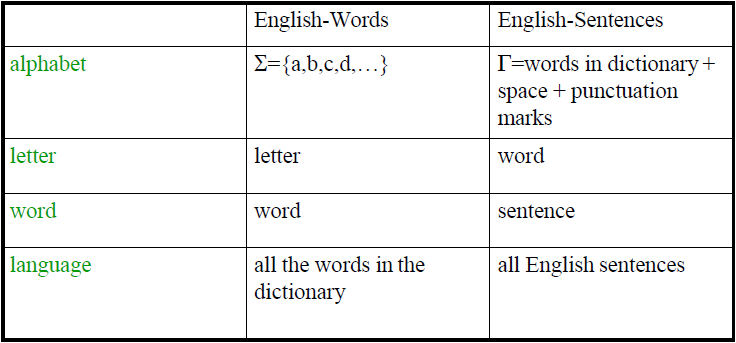
\includegraphics[width=\linewidth]{lectures/figures/definitions.png}
    \caption{Examples of the definitions.}
\end{figure}

Two words are considered the same if all their letters are the same and in the same order.
There is a difference between the word that has no letters $(\Lambda)$, and the language that has no words $(\Phi)$.
It is not true that $\Lambda$ is a word in the language $\Phi$ since this language has no words at all.

Languages can be defined as a list of all of the words, or as a set of the rules \textbf{(grammar)}. The alphabet is always finite, but the set of words can be infinite. It must be possible in a finite time to determine if a word is in a language or not (algorithm).

\begin{align*}
    \Sigma={x} &\ \ L_1=\{x,xx,xxx,xxxx,\ldots\}\\
    &\text{or}\\
    &\ \ L_1 = \{X^n | n = 1,2,3,\ldots\}
\end{align*}

Concatenation is when two words, written down side by side, create a new word:
\begin{align*}
    a&=xxx & b&=xxx & ab&=xxxxx
\end{align*}
When a word is concatenated, we are able to factor out the individual words.

\begin{align*}
    \Sigma&=\{0,1,2,3,4,5,6,7,8,9\}\\
    L_2&=\{\text{words that do not start with the letter} 0\}
\end{align*}

Length is the number of letters in a word:
\begin{align*}
    \text{length}(xxxxx)&=5\\
    \text{length}(1025)&=4\\
    \text{length}(\Lambda)&=0
\end{align*}
Reverse will reverse the letters in a word:
\begin{align*}
    \text{reverse}(xxx)&=xxx\\
    \text{reverse}(1570)&=751
\end{align*}
A palindrome is a word that is the same reading forwards as it is reading backwards:
\begin{align*}
    \Sigma&=\{a,b\}\\
    \text{Palindrome}&:=\{\Lambda \text{ and } x | \text{reverse}(x) = x\}\\
    &=\{\Lambda, a, b, aa, bb, aaa, aba, bab, bbb, \ldots\}
\end{align*}

\subsection{Kleene Closure (Star)}
Given an alphabet \(\Sigma\), the closure of \(\Sigma\) (or Kleene star), denoted as \(\Sigma^*\), is the language containing all words made up of finite sequences of letters from \(\Sigma\), including the empty string \(\Lambda\).
\begin{align*}
    \Sigma&=\{x\} & \Sigma^*&=\{\Lambda, x, xx, xxx,\ldots\}\\
    \Sigma&=\{0,1\} & \Sigma^*&=\{\Lambda,0,1,00,01,10,11,000,001,\ldots\}\\
    \Sigma&=\{a,b,c\} & \Sigma^*&=\{\Lambda,a,b,c,aaa,aab,aac,aba,abb,abc,\ldots\}
\end{align*}
Let \(S\) be a set of words. \(S^*\) is the language formed by concatenating words from \(S\), including the empty string (null string) \(\Lambda\).
\begin{align*}
    S&=\{a,ab\} & S^*&=\{\Lambda,a,aa,ab,aaa,aab,aba,aaaa,\ldots\}
\end{align*}
\[
    abaaababa \in S^*
\]
\[
    ab|a|a|ab|ab|a \leftarrow \text{factors}
\]
\begin{align*}
    S^*=\{&\Lambda \text{ plus all sequences of a's and b's except those}\\
    &\text{that start with b and those that contain a double b}\}
\end{align*}
Factoring is not always unique, if \(S=\{xx,xxx\}\) and \(xxxxxxx \in S^*\), then there are multiple ways to break up the word between the words in \(S\).

The Kleene closure of an alphabet \(\Sigma\) always produces an infinite language unless \(\Sigma\) is empty. Only for infinite languages, the Kleene closure of two sets can end up being the same language even if the two sets started with were not.
\begin{align*}
    S &= \{a,b,ab\} & T &= \{a, b, bb\} & S^* &= T^*
\end{align*}

\subsection{Positive Closure (Plus)}
The language with all concatenations that contain at least one word from \(S\) and one letter from \(\Sigma\).\\
(\(S^*\) possibly without \(\Lambda\).)

If \(\Lambda\) is a member of \(S\), \(S^* = S+\).

\textbf{Equality of sets}\\
\(S=T\): \ \(S \subset T\) and \(T \subset S\)

\textbf{Subsets}\\
\(S \subset T\): for all \(x\) in \(S\), \(x\) is also in \(T\).

\begin{theorem}
    For any set of words \(S\), we have \(S^{**}=S^*\).
\end{theorem}
\begin{proof}
    \textbf{Case 1:} \(S^{**} \subset S^*\)\\
    Every word in \(S^{**}\) is made up of factors from \(S^*\) (definition of Kleene star). Every word in \(S^*\) is made up of factors from \(S\). Therefore every word in \(S^{**}\) is made up of factors from \(S\).\\
    \textbf{Case 2:} \(S^* \subset S^{**}\)\\
    For any set A, we can show that \(A \subset A^*\). Let \(w\) be a word in \(A\). Then \(w\) is certainly in \(A^*\). If we consider \(S^*\) as our set \(A\), we can conclude \(S^* \subset S^{**}\).\\
    By definition of equality of sets, we have \(S^* = S^{**}\).
\end{proof}